\documentclass[fleqn,dvipdfmx]{jarticle}
\usepackage[a4paper,top=3cm,bottom=2cm,left=2cm,right=2cm]{geometry}
\NeedsTeXFormat{pLaTeX2e} 
\everymath{\displaystyle} 
\usepackage[dvipdfmx]{graphicx} 
\usepackage[svgnames]{xcolor} 
\usepackage{amsmath,amssymb,amsthm,ascmac,mathtools,ulem,tcolorbox,enumerate,pdfpages,multicol,tikz,here,mathcomp,graphics,url} 
\usetikzlibrary{intersections, calc} 
\tcbuselibrary{breakable, skins, theorems}
\renewcommand{\qedsymbol}{$\blacksquare$}

\title{電気電子計測 事前レポート}
\author{3309 大山 主朗}
\date{}
\begin{document}
\maketitle
\section{真値と誤差および相対誤差(誤差率)}
\textbf{真値}(true value)とは測定値の真の値,\textbf{誤差}(error)は真値と測定値の差のことである.
真値への補正量を\textbf{補正値}(correction)という.
誤差$\varepsilon$,補正値$\alpha$,測定値$M$,真値$T$には以下の関係がある.~[1]\\
\begin{align}
	\varepsilon &=M-T\\
	\alpha &=T-M=-\varepsilon
\end{align}
 しかしながら,真値は不明なことが多く,代替として平均値(mean)や理論値(theoretical value)を用いている.誤差や補正を比を用いて表現する方法を以下にまとめる. \\
\begin{enumerate}
	\item \textbf{誤差率}(error rate)・\textbf{相対誤差}(relative error):
	\begin{equation}
	\frac{\varepsilon}{T}
	\end{equation}
	\item \textbf{誤差百分率}(percentage error):
	\begin{equation}
		\frac{\varepsilon}{T}\times 100[\%]
	\end{equation}
	\item \textbf{補正率}(correction facter
		)・\textbf{相対補正}(relative correction):
	\begin{equation}
		\frac{\alpha}{M}
	\end{equation}
	\item \textbf{補正百分率}(percentage correction):
	\begin{equation}
		\frac{\alpha}{M}\times 100[\%]
	\end{equation}
\end{enumerate}


 誤差には種類があり,それいより補正の仕方なども変わる.
\begin{enumerate}
	\item \textbf{間違い}(mistake):\\
		 読み間違い,記録違い,計器の不整備などの不注意により生じる誤差であり,再測定,理論値との比較などを行うことで除くことが可能.
	\item \textbf{系統誤差}(system error):\\
		 計器自体が持っている誤差(\textbf{器差}(insturumental error)),測定環境に夜誤差,測定器による誤差,個人差などによるかたよりなど.補正できるものがほとんどであり,測定器のカタログ・マニュアルに掲載されている誤差はほとんどこれである.
	\item \textbf{偶然誤差}(random error):\\
		 原因不明や,わかっていても除くことのできない誤差.\textbf{熱雑音}(thermal noise)は室温で実験している限り必ず混入する雑音で,偶然誤差の代表的なものである.この誤差はランダムであるとされ,統計的手法により測定値を推定することができる.\\
		参考に,抵抗の内部で発生する雑音の電圧$V_n[V]$を以下に示す.~[2]
		\begin{align*}
			V_n&=\sqrt{4k_BTR\Delta f}\\
			k:ボルツマン定数[J/K],&\quad T:絶対温度[K]\\
			R:抵抗値[\Omega],&\quad\Delta f:帯域[Hz]
		\end{align*}
	\item \textbf{相対誤差}(relative error)~[3]:\\
		 誤差と真値との比のことで,単位の異なる物理量の不確かさを比較したり,乗除算による誤差の伝播を議論する際に用いられる.「測定値が1\%の誤差を含む」などという場合の「1\%」が相対誤差である.
\end{enumerate}


\section{統計処理(正規分布・平均値・標準偏差)}~[3]
\begin{enumerate}
\item \textbf{平均値}(mean)\\
平均値$\overline{x}$は測定値$x_1,x_2,\cdots x_n$とすると平均値は次式となる.
		\begin{equation}
			\label{7}
			\overline{x}=\frac{1}{n}\sum_{i=1}^{n} x_i
		\end{equation}
式\ref{7}は算術平均と呼ばれるものであり,他にも平均値には幾何学平均や調和平均,トリム平均などがある.\\
		\textbf{幾何学平均}(geometric mean)は式\ref{8}で定義され,比率や割合で変化するものに対してその平均を求めるときに用いられる.~[4]
		\begin{equation}
			\label{8}
			\overline{x}_G=\sqrt[n]{x_1x_2\cdots x_n}
		\end{equation}
		\textbf{調和平均}(harmonic mean)は式(\ref{9})で表され,速度の平均などを求める際に利用される.
		\begin{equation}
			\label{9}
			\overline{x}_H=\frac{n}{\sum_{i=1}^n \frac{1}{x_i}}
		\end{equation}
		\textbf{トリム平均}(Truncated mean)はデータを小さい順に並べた時,小さい側と大きい側からそれぞれ指定した個数の値(ここでは$k$個)を除き,残ったデータのみから求める平均のことで,式\ref{10}で表される.
		\begin{equation}
			\overline{x}_k=\frac{1}{n-2k}\sum_{i=1+k}^{n-k} x_i
		\end{equation}

\item \textbf{標準偏差}(standard deviation)\\
 測定値と母平均の差を\textbf{偏差}(deviation)といい,偏差の2乗和平均$u$を\textbf{分散}(variance),その平方根を標準偏差$\sigma$といい次式で表す.
		\begin{equation}
			\label{11}
			u=\sigma^2=\frac{1}{n}\sum_{i=1}^n (x_i-\mu)^2
		\end{equation}
		\textbf{母平均}(population mean)$\mu$と\textbf{標本平均}(sample mean)$\overline{x}$は異なる値であるが,標本の数を増加させると,標本平均も母平均に近づく.このように,$n \to \infty$で標本のパラエータが母集団のパラメータに一致する物を\textbf{不偏推定量}(unbiased estimator)という.式\ref{11}で,$\mu$の代わりに$1/(n-1)$とした際の分散を\textbf{標本分散}(sample variance)といい,$\sigma$の不偏推定量である.

\item \textbf{正規分布・ガウス分布}(normal distribution・Gaussian distribution)~[6]\\
 同一条件下での測定値が$x$と$x+dx$の間にある\textbf{確率密度}(probability density):ある値の相対的な出やすさは正規分布に従うとされ,\textbf{確率密度関数}(probability density function)は以下のようになる.(\ref{12})
	\begin{equation}
	\label{12}
	f(x)dx=\frac{1}{\sqrt{2\pi}\sigma} \exp \left\{-\frac{(x-\mu)^2}{2\sigma^2}\right\}dx
	\end{equation}
 確率密度とは,定義域内での$X$の値の「相対的な出やすさ」を表すものである.また,確率密度関数は連続型確立変数$X$がある値$x$をとる関数$f(x)$のことで,$X=x$となる確率密度関数は以下のように表すことができる.(\ref{13})\\
\begin{equation}
\label{13}
f(x)=f(X=x)
\end{equation}
 正規分布は最も代表的な分布の一つで,反復試行の成功回数などが従う確率分布も(近似的に)これとなる.~[7]\\
 図\ref{plot1}にgnuplotによる正規分布を示す.ここで全事象の和の確率が$1$となることを,式(\ref{14})で確認する.\\
また,正規分布において$[-\sigma,\sigma]$に入る確率は約$68[\%]$,$[-2\sigma,2\sigma]$に入る確率は約$95[\%]$である.
\begin{align}
\label{14}
&\int_{-\infty}^{\infty} f(x)\,dx\nonumber\\
=&\frac{1}{\sqrt{2\pi}\sigma} \int_{-\infty}^{\infty} \exp \left(\frac{(x-\mu)^{2}}{2\sigma^{2}}\right)dx\nonumber\\
ここで,&x-\mu=yと置換すると,上式は,\nonumber\\
=&\frac{1}{\sqrt{2\pi}\sigma } \int_{-\infty}^{\infty} \exp \left(-\frac{y^{2}}{2\sigma^{2}}\right)dy\nonumber\\
=&\frac{1}{\sqrt{2\pi}\sigma }\sqrt{2\sigma^{2}\pi}=1
\end{align}
\begin{figure}[htbp]
\centering
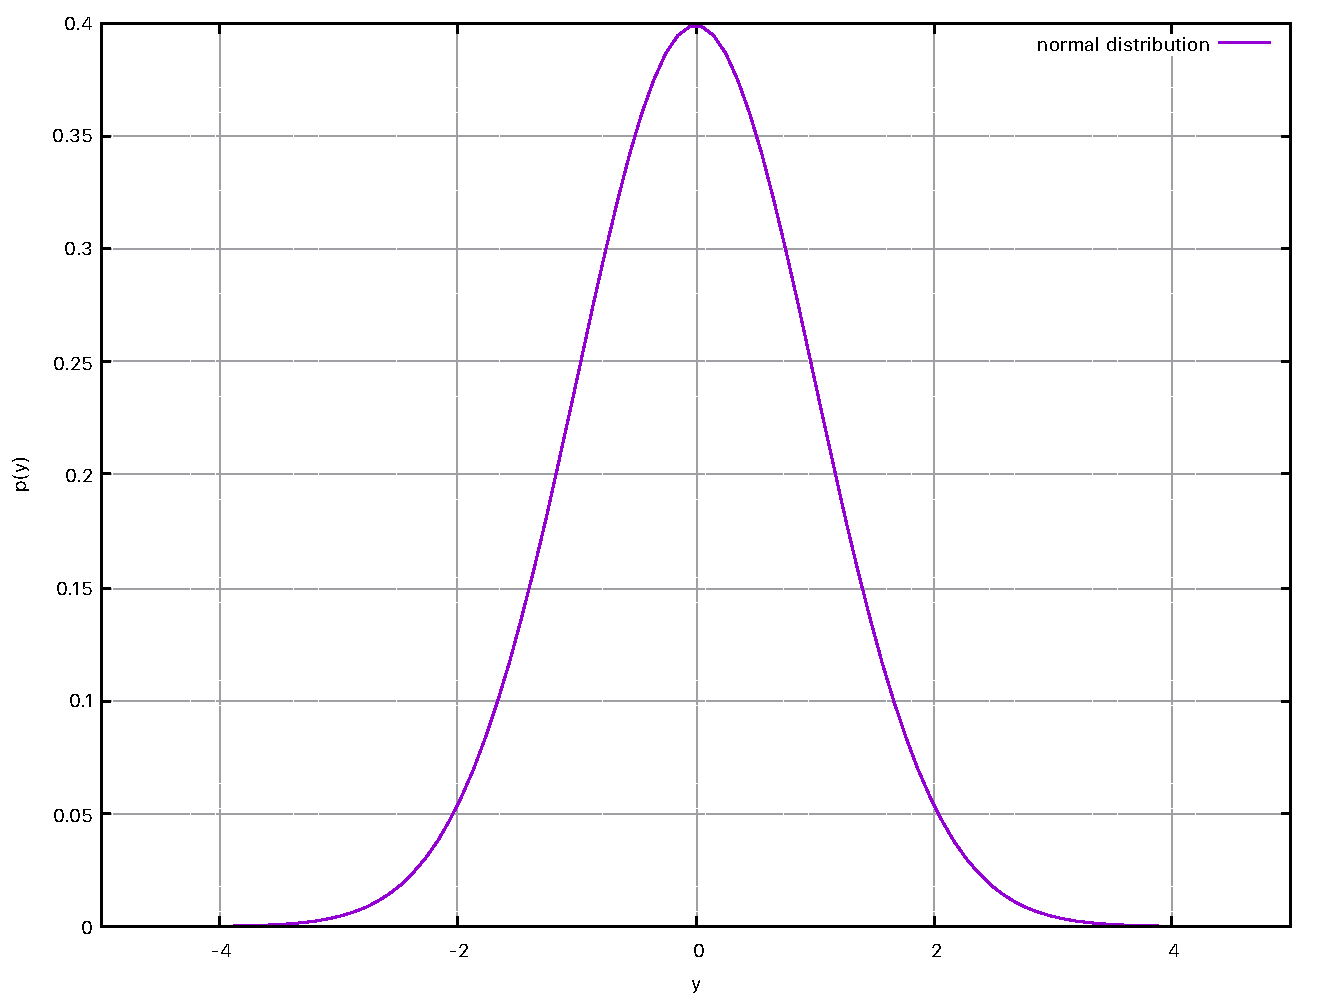
\includegraphics[scale=0.8]{./plot.pdf}
\caption{正規分布}
\label{plot1}
\end{figure}
\end{enumerate}



\section{散布図の回帰分析(線形回帰・最小二乗法)}
\textbf{回帰分析}(regression analysis)は結果となる数値と要因となる数値の関係を調べ,それぞれの関係を明らかにするものである.この時,要因となる数値を\textbf{説明変数},結果となる数値を\textbf{被説明変数},そしてそれらに対する関数を\textbf{目的関数}という.\\
 目的関数が線形あるいは,それに近いものを\textbf{線形回帰}(linear regression)という.実用として,回帰分析は,事象の予測・シミュレーション・検証・要因分析などで用いられ一般に
\begin{align}
単回帰:y&=a+bx\\
重回帰:y&=\sum_{i=1}^{n} a+b_{i}x_{i}
\end{align}
の式で表される.~[8]\\
 \space\textbf{最小二乗法}(method of least squares)は回帰分析の1つで,測定データの組みから,ある関数を用いて近似するとき,その関数が測定値に対してよい近似となるように残差(測定値と近似曲線の差)の二乗和が最小となるように係数を決定する方法のことである.\\
 以下に,$n$回の測定よって得られたデータ$(x_{1},y_{1})\cdots(x_{n},y_{n})$があり式\ref{15}のような線形関係が成り立っているとした場合の最小二乗法を用いる過程を示す.
\begin{equation}
\label{15}
Y=ax+b
\end{equation}

\begin{shadebox}
\begin{align*}
\varepsilon_{1}&=y_{1}-Y_{1}=y_{1}-ax_{1}-b\\
\varepsilon_{2}&=y_{2}-Y_{2}=y_{2}-ax_{2}-b\\
\vdots\\
\varepsilon_{n}&=y_{n}-Y_{n}=y_{n}-ax_{n}-b\\
\\
\varepsilon_{i}の&2乗和が最小になるa,bは,次の方程式を満足する.\\
a\sum_{i=1}^{n}x_{i}&+nb=\sum_{i=1}^{n}y_{i}\\
a\sum_{i=1}^{n}x_{i}^{2}&+b\sum_{i-1}^{n}x_{i}=\sum_{i=1}^{n}x_{i}y_{i}\\
\\
以上より,&係数a,bは\\
a&=\frac{\Sigma (y_{i}-\overline{y}x_{i})}{\Sigma (x_{i}-\overline{x})^{2}}\\
b&=\overline{y}-a\overline{x}
\end{align*}
\end{shadebox}


\begin{thebibliography}{9}
\item 阿部武雄/村山実, ``電気・電子計測【第4版】", 1.3.1, 森北出版, 2022
\item 進工業株式会社, \url{https://www.susumu.co.jp/tech/know_how_04.php}, 2022/05/01
\item 阿部武雄/村山実, ``電気・電子計測【第4版】", 1.4.3, 森北出版, 2022
\item 武内修, \url{https://dora.bk.tsukuba.ac.jp/~takeuchi/?%E3%81%AF%E3%81%98%E3%82%81%E3%81%A6%E3%81%AE%E8%AA%A4%E5%B7%AE%E8%AB%96#a2360208}, 2022/05/01
\item 統計WEB, \url{https://bellcurve.jp/statistics/course/4324.html}, 2022/05/01
\item 統計WEB, \url{https://bellcurve.jp/statistics/course/6602.html}, 2022/05/02
\item 高校数学の美しい物語, \url{https://manabitimes.jp/math/931}, 2022/05/02
\item 埼玉県, \url{https://www.pref.saitama.lg.jp/a0206/toukeifaq/q7-1.html}, 2020/05/03
\item 阿部武雄/村山実, ``電気・電子計測【第4版】", 1.4.4, 森北出版, 2022
\end{thebibliography}
\end{document}
